%! TEX root = lecture/Complex_Analysis

\subsection{The Riemann Zeta Function}
We proved in homework that the Riemann zeta function 
\begin{equation}
    \zeta(s)=\sum_{n=1}^\infty\frac{1}{n^s},\,s=\sigma+it
\end{equation}
is analytic in the half-plane  $ \Re s>1 $.
\begin{theorem}
    $ \zeta  $ has the following properties:
    \begin{enumerate}[label=(\alph*)]
        \item (Euler product formula)  $ \zeta  $ has the infinite product representation   \[\zeta(s)=\dps\prod_{p \text{ prime}}\frac{1}{1-p^{-s}},\, \Re s>1 \]
        \item  $ \zeta  $ extends to a meromorphic function on  $ \Cbb $ whose only poly is a simple pole at  $ s=1 $  with residue  $ 1 $.
        \item  $ \zeta  $ has no zeros in  $ \Re s \geq 1 $, all zeros of  $ \zeta $ in  $ \Re s \leq 0 $ are at  $ s=-2k $,  $ k\in \Nbb $. 
        \item  $ \zeta(2n)=\dps\frac{(-1)^{n-1}(2\pi )^{2n}}{2\cdot(2n)!}B_{2n} $,  $ n\in \Nbb $ where  $ B_{n} $ are the Bernoulli numbers, defined by  \[\dps\frac{z}{e^z-1}=\sum_{m=0}^\infty\frac{B_m}{m!}z^m ,\,|z|<2\pi \] 
        and  $ \zeta(-n)=-\dps\frac{B_{n+1}}{n+1},\,n\in \Nbb $.
        \item  $ \zeta  $ satisfies the functional equation  $ \zeta^*(1-s)=\zeta^*(s) $ where  $ \zeta^*  $ is the \name{symmetrized zeta function} defined by 
        \begin{equation}\label{eq:5.4:symmetrized zeta function}
            \zeta^*(s)=\pi^{-\frac{s}{2}}\Gamma(\frac{s}{2})\zeta(s)
        \end{equation}
        \item  $ \zeta^*(s)=\dps-\frac{1}{1-s}-\frac{1}{s}+\frac{1}{2}\int_1^\infty (t^{-\frac{s+1}{2}}+t^{\frac{s-2}{2}})(\theta(t)-1)\dd t $,  $ s\in \Cbb\setminus\{0,1\} $, where  $ \theta  $ is one of the \name{Jacobi theta series}, defined as 
        \begin{equation}\label{eq:5.4:Jacobi theta series}
            \theta(t)=\sum_{n=-\infty}^\infty e^{-\pi n^2t}
        \end{equation}
        \item  $ \zeta(s)=\dps\frac{\Gamma(1-s)}{2\pi i}\int_C\frac{(-z)^s}{e^z-1}\cdot\frac{\dd z}{z} $ where  $ C  $ is the contour shown in the picture, with  $ \epsilon<2\pi $,  $ (-z)^s=\exp[s\ln (-z)] $,  $ \ln(-z) $ is chosen \st  $ -\pi <\Im \ln (-z)<\pi $.        
        

       \begin{center}
        \tikzset{every picture/.style={line width=0.75pt}} %set default line width to 0.75pt        

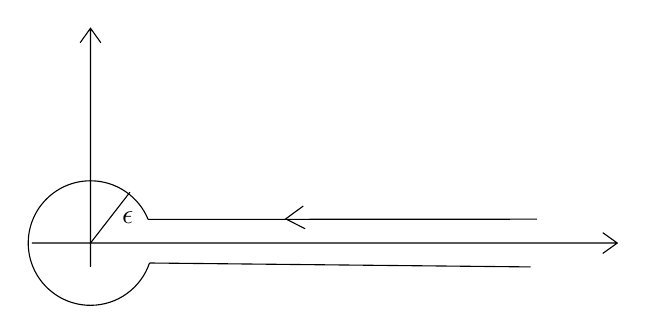
\begin{tikzpicture}[x=0.75pt,y=0.75pt,yscale=-1,xscale=1]
%uncomment if require: \path (0,300); %set diagram left start at 0, and has height of 300

%Shape: Axis 2D [id:dp9785911867399795] 
\draw  (220.8,168.5) -- (502.8,168.5)(249,65) -- (249,180) (495.8,163.5) -- (502.8,168.5) -- (495.8,173.5) (244,72) -- (249,65) -- (254,72)  ;
%Shape: Arc [id:dp1302548314750347] 
\draw  [draw opacity=0] (277.43,178.11) .. controls (273.42,189.96) and (262.21,198.5) .. (249,198.5) .. controls (232.43,198.5) and (219,185.07) .. (219,168.5) .. controls (219,151.93) and (232.43,138.5) .. (249,138.5) .. controls (261.53,138.5) and (272.27,146.18) .. (276.76,157.1) -- (249,168.5) -- cycle ; \draw   (277.43,178.11) .. controls (273.42,189.96) and (262.21,198.5) .. (249,198.5) .. controls (232.43,198.5) and (219,185.07) .. (219,168.5) .. controls (219,151.93) and (232.43,138.5) .. (249,138.5) .. controls (261.53,138.5) and (272.27,146.18) .. (276.76,157.1) ;  
%Straight Lines [id:da7349516742118151] 
\draw    (276.76,157.1) -- (464,157) ;
%Straight Lines [id:da49149077320950185] 
\draw    (277.43,178.11) -- (461,180) ;
\draw   (351.53,150.65) -- (343.02,156.87) -- (352.44,161.61) ;
%Straight Lines [id:da007165525380332216] 
\draw    (249,168.5) -- (268,144) ;

% Text Node
\draw (263,152) node [anchor=north west][inner sep=0.75pt]   [align=left] {$\displaystyle \epsilon $};


\end{tikzpicture}

       \end{center}
        

    \end{enumerate}
\end{theorem} 
\begin{proof}\,

    $ \dps\prod_{p\text{ prime}}\frac{1}{1-p^{-s}}=\frac{1}{\dps \prod_{p\text{ primes}}(1-p^{-s})} $,  $ \Re s>1 $ converges absolutely since  $ \dps\sum_{p\text{ prime}}|p^{-s}|=\sum_{p\text{ prime}}p^{-\Re s} $ converges for  $ \Re s>1 $. Hence,  $ F(s)=\dps\prod_{p\text{ prime}}\frac{1}{1-p^{-s}} $ is analytic and nonzero in  $ \Re s>1 $. It remains to prove that  $ \zeta(s)=F(s) $ for  $ \Re s>1 $.
    \begin{align*}
        \zeta_N(s)&:=\prod_{p \leq N,p\text{ prime}}\frac{1}{1-p^s}\\
        &=\prod_{p \leq N,p\text{ prime}}\sum_{k=0}^\infty p^{-ks}\\
        &=\sum_{\substack{n=p_1^{k_1}p_2^{k_2}\cdots p_m^{k_m}\\p_j \leq N,p_j\text{ prime}}}\frac{1}{n^s},\,\Re s>1
    \end{align*}  
    By the fundamental theorem of arithmetic, 
    \[|\zeta(s)-\zeta_N(s)| \leq \sum_{n \geq N}\frac{1}{|n^s|}\rightarrow 0\text{ as }N\rightarrow \infty\]
    which proves (a), and part of (c):  $ \zeta  $ has no zeros in  $ \Re s>1 $.
    
    Define  $ \dps\theta(t)=\sum_{n=-\infty}^\infty e^{-\pi n^2t} $. We next prove that  $ \theta(t)=\dps\frac{1}{\sqrt{t}}\theta(\frac{1}{t}) $,  $ \forall t>0 $.
    
    $ f(x)=exp(-\pi +x^2) $ whose Fourier transform is 
    \[\hat{f}(k)=\int_{-\infty}^\infty f(x)\exp[-2\pi i kx]\dd x=\frac{1}{\sqrt{t}}\exp[-\frac{\pi k^2}{t}]\]
    The Poisson summation formula implies  \begin{equation}\label{eq1:5.4:theta(t)}
        \theta(t)=\dps\sum_{n=-\infty}^\infty e^{-\pi n^2t}=\sum_{n=-\infty}^\infty \frac{1}{\sqrt{t}}\exp[-\frac{\pi k^2}{t}]=\frac{1}{\sqrt{t}}\theta(\frac{1}{t})
    \end{equation} 
    Note that  $ \theta(t)-1=2\dps\sum_{n=1}^\infty e^{-\pi n^2 t} \leq 2\sum_{n=1}^\infty e^{-\pi nt}=2\frac{e^{-\pi t}}{1-e^{-\pi t}} $,  $ \forall t>0 $.

    \ie  $ \theta(t)=1+O(e^{-\pi t}) $   as  $ t\rightarrow \infty  $.
    
    \eqref{eq1:5.4:theta(t)} implies  $ \dps\theta(t)=\frac{1}{\sqrt{t}}[1+O(e^{-\pi/t})] $ as  $ t\rightarrow 0^+ $ $ \Rightarrow  $  $ \dps\theta(t)=O(\frac{1}{\sqrt{t}}) $  as  $ t\rightarrow 0^+ $.
    
    \begin{equation}
        \Gamma(\frac{s}{2})=\int_0^\infty e^{-t}t^{\frac{s}{2}-1}\dd t,\,\Re s>1
    \end{equation}
    Then replace  $ t  $ with  $ \pi n^2 t $. We obtain that  
    \begin{equation}
        \pi^{-\frac{s}{2}}\Gamma(\frac{s}{2})n^{-s}=\int_0^\infty e^{-\pi n^2t}t^{\frac{s}{2}-1}\dd t,\,\Re s>1
    \end{equation}
    Summing over  $ n $ $ \Rightarrow  $   
    \begin{equation}
        \begin{aligned}
            \zeta^*(s)&=\dps\sum_{n=1}^\infty \int_0^\infty e^{-\pi n^2t}t^{\frac{s}{2}-1}t^{\frac{s}{2}-1}\dd t\\
            & \xlongequal{Fubini} \int_0^\infty \left(\sum_{n=0}^\infty e^{-\pi n^2t}\right)t^{\frac{s}{2}-1}\dd t\\
            &=\int_0^\infty\frac{\theta(t)-1}{2}t^{\frac{s}{2}-1}\dd t,\,\Re s>1
        \end{aligned}
    \end{equation}
    Define  $\dps g(t)=\frac{\theta(t)-1}{2} $. Then  $ g(t)=\dps\frac{\frac{1}{\sqrt{t}}\theta(\frac{1}{t})-1}{2}=\frac{1}{\sqrt{t}}g(\frac{1}{t})+\frac{1}{2\sqrt{t}}-\frac{1}{2} $. Therefore, 
    \begin{equation}
        \begin{aligned}
            \zeta^*(s)&=\int_0^1g(t)t^{\frac{s}{2}-1}\dd t+\int_1^\infty g(t)t^{\frac{s}{2}-1}\dd t\\ 
            &=\int_0^1[\frac{1}{\sqrt{t}}g(\frac{1}{t})+\frac{1}{2\sqrt{t}}-\frac{1}{2}]t^{\frac{s}{2}-1}\dd t+\int_1^\infty g(t)t^{\frac{s}{2}-1}\dd t\\ 
            &=-\frac{1}{s}-\frac{1}{1-s}+\frac{1}{2}\int_1^\infty[\theta(t)-1]\cdot[t^{\frac{-s-1}{2}}+t^{\frac{s}{2}-1}]\dd t,\,\Re s>1
        \end{aligned}
    \end{equation}
    which is analytic if we apply Weierstrass theorem to the final integral. So  $ \zeta  $ can be extended to a meromorphic function on  $ \Cbb $, whose poles are  $ 0,1 $.
    
    \eqref{eq:5.4:symmetrized zeta function} implies  $ \zeta^*(s)=\zeta^*(1-s) $.
    
    This combined with Legendre's duplication formula and  $ \dps\frac{1}{\Gamma(1-\frac{s}{2})\Gamma(\frac{s}{2})}=\frac{\sin (\pi \frac{s}{2})}{\pi} $, we obtain that 
    \begin{equation}\label{eq:5.4:symmetry of zeta function}
        \zeta(s)=2^s\pi^{s-1}\sin(\frac{\pi s}{2})\Gamma(1-s)\zeta(1-s),\, s\in \Gamma\setminus\{0,1\}
    \end{equation} 

    $ \zeta^* $ has simple poles at  $ s=0 $ and  $ s=1 $, with residues  $ -1 $ and  $ 1 $ respectively.
    
    $ \zeta(s)=\dps\frac{\pi^{\frac{s}{2}}\zeta^*(s)}{\Gamma(\frac{s}{2})} $ $ \Rightarrow  $  $ \zeta  $ has a simple pole at  $ s=1 $ with residue  $ \dps\frac{\pi^{\frac{1}{2}}}{\Gamma(\frac{1}{2})}=1 $.  $ s=0 $ is a removable singularity since  $ \Gamma(s)=\dps\frac{1}{s} $ as  $ s\rightarrow 0 $. And  $ \zeta(0)=\dps\frac{1\cdot\frac{-1}{s}}{\frac{1}{\frac{s}{2}}}=-\frac{1}{2} $.   
    
    \eqref{eq:5.4:symmetry of zeta function} implies zeros of  $ \zeta $ for  $ \Re s<0 $ are precisely  $ s=-2k $,  $ k\in \Nbb $.
    
    We have proved (b),(c),(e),(f).

    We next prove (g).
    \begin{align*}
        \int_0^\infty\frac{t^{s-1}}{e^t-1}\dd t&=\int_0^\infty t^{s-1}\sum_{n=1}^\infty e^{-nt}\dd t\\
        &\xlongequal{{Fubini}}\sum_{n=0}^\infty\int_0^\infty t^{s-1}e^{-nt}\dd t\\
        &\overset{u=nt }{=}\sum_{n=1}^\infty\frac{1}{n^s}\int_0^\infty u^{s-1}e^{-u}\dd u\\
        &=\Gamma(s)\zeta(s),\,\Re s>1
    \end{align*}
    For  $ \dps\int_C\frac{(-z)^s}{e^z-1}\cdot\frac{\dd z}{z},\,\Re s>1 $, as  $ \epsilon\downarrow 0 $, the contribution from the  circle of radius  $ \epsilon $ $ \rightarrow 0 $.  Then 
    \begin{align*}
        \int_C\frac{(-z)^s}{e^z-1}\cdot\frac{\dd z}{z}&=\int_{-\infty}^0\frac{\exp[s(\ln t-i\pi)]}{e^t-1}\cdot\frac{dd t}{t}+\int_0^\infty \frac{\exp[s(\ln t+i\pi)]}{e^t-1}\cdot\frac{\dd t}{t}\\
        &=(e^{is\pi}-e^{-is\pi})\int_0^\infty\frac{t^{s-1}}{e^t-1}\dd s\\
        &=2i\sin(s\pi)\Gamma(s)\zeta(s),\,\Re s>1
    \end{align*}  
    \begin{equation}\label{eq:5.4:another expandation of zeta function}
        \begin{aligned}
            \Rightarrow \zeta(s)&=\frac{1}{2i\sin(s\pi)\Gamma(s)}\int_C\frac{(-z)^s}{e^z-1}\cdot\frac{\dd z}{z}\\
            &=\frac{\Gamma(z-s)}{2\pi i}\int_C\frac{(-z)^s}{e^z-1}\cdot\frac{\dd z}{z},\,\Re s>1
        \end{aligned}  
    \end{equation}

    For (d), for  $ \forall n\in \Nbb $,
    \begin{equation}
        \begin{aligned}
            \zeta(-n)&\overset{\eqref{eq:5.4:another expandation of zeta function}}{=}\frac{\Gamma(1+n)}{2\pi i}\int_C\frac{(-z)^{-n}}{e^z-1}\dd z\\
            &=\frac{n!}{2\pi i}\int_C\frac{(-z)^{-n}}{z^2}\sum_{m=0}^\infty\frac{B_m}{m!}z^m\dd z\\
            &=n!(-1)^n\frac{B_{n+1}}{(n+1)!}\\
            &=\frac{}{}
        \end{aligned}
    \end{equation} 
\end{proof}